\begin{figure}
   \begin{subfigure}{\textwidth}
      {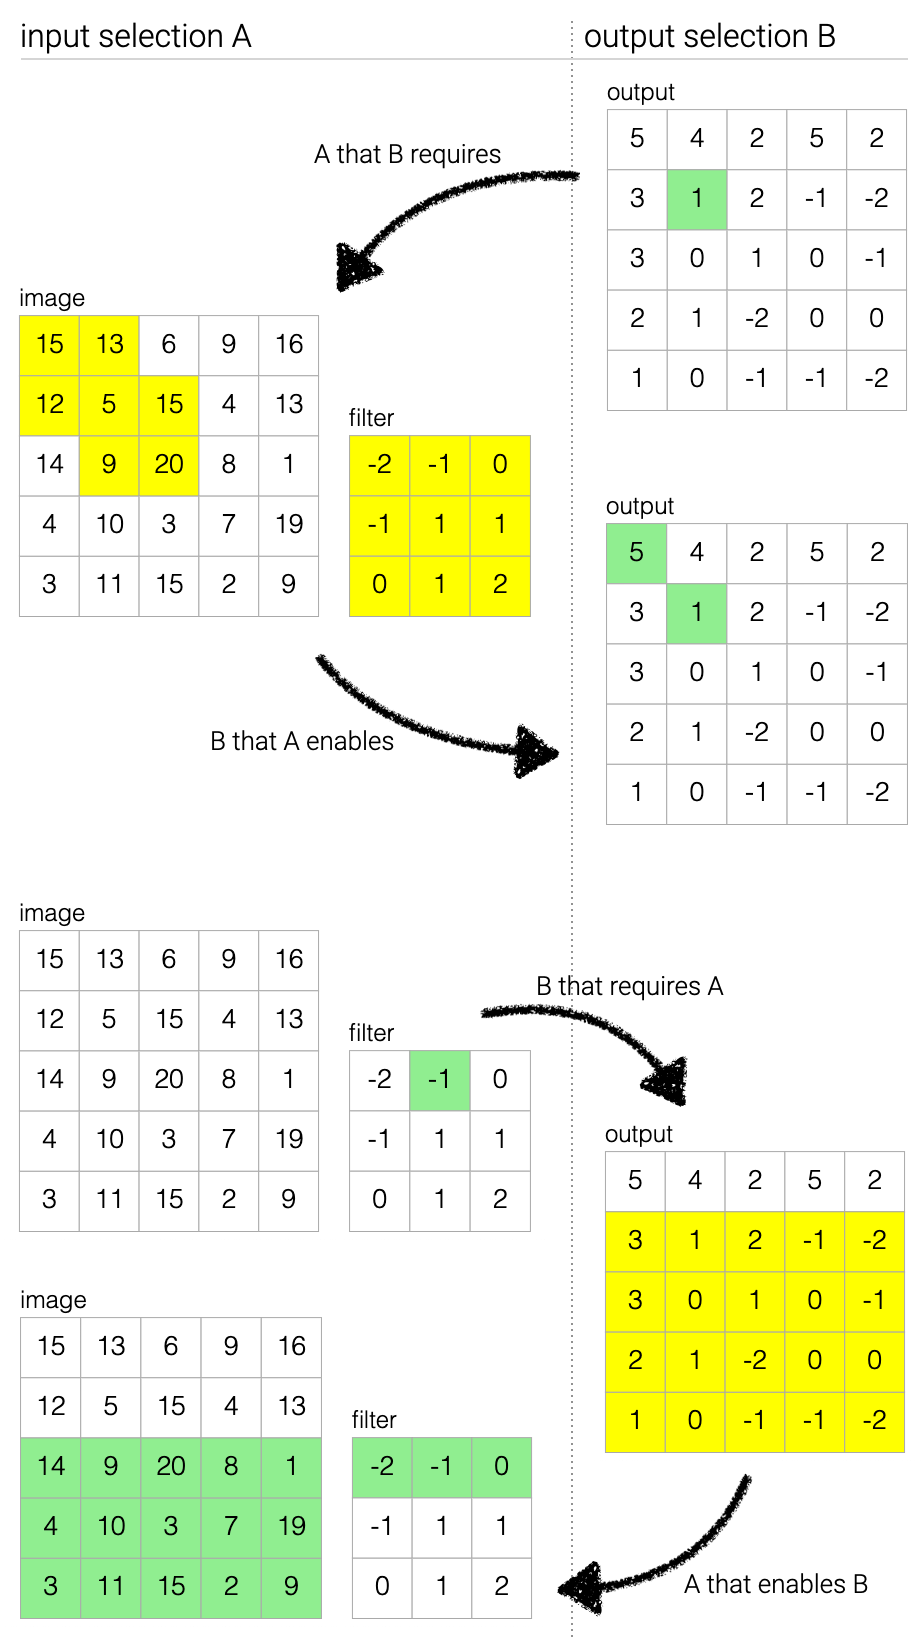
\includegraphics[scale=0.4]{fig/example/4-relations.png}}
      \caption{4 dependency relations}
   \end{subfigure}
   \begin{subfigure}{0.48\textwidth}
      \small
      \lstinputlisting[language=Fluid]{fluid/convolution.fld.mod}
   \end{subfigure}
   \begin{subfigure}{0.48\textwidth}
      \small
      \lstinputlisting[language=Fluid]{fluid/conv-edgeDetect.fld.mod}
   \end{subfigure}
   \caption{Matrix convolution example}
\end{figure}
